\documentclass[review,3p,times,authoryear,12pt]{elsarticle}
\usepackage{amsmath,amsthm,amssymb}
\usepackage{algorithm}
\usepackage{graphicx,subfigure}
\usepackage{clrscode3e}
\usepackage{enumerate}
\usepackage{multirow,endfloat}
\graphicspath{{figure/}}
\newtheorem{proposition}{Proposition}


\begin{document}
\begin{frontmatter}
\newpage

\title{A Heuristic and Algorithm Bound for the Stowage Stack Minimization Problem with K-Rehandle Constraint}
%\author[shu]{Ning Wang\corref{corl}}
%%\ead{ningwang@shu.edu.cn}
%
%\author[shu]{Shanhui Ke}
%
%%\author[syu]{Zizhen Zhang}
%
%\author[set]{Bo Wang}
%
%
%\address[shu]{
%Department of Information Management, School of Management, Shanghai University, Shanghai, China
%}
%%\address[syu]{
%%School of Data and Computer Science, Sun Yat-Sen University, China
%%}
%\address[set]{
%College of Urban Rail Transportation, Shanghai University of Engineering Science, China
%}
%\cortext[corl]{Corresponding author. E-mail: ningwang@shu.edu.cn. Address: No. 333, Nanchen Road, Shanghai, China, 200444}%zhangzizhen@gmail.com

\begin{abstract}
<<<<<<< HEAD
The Stowage Stack Minimization Problem (SSMP) investigates a stowage planning problem when carriers have the obligation to ship all the given containers from/to different ports, with the objective to utilize the fewest number of stacks on the ship. This problem has realistic usefulness since it can help shipping forwarders estimate the shipping space of each shipper.
To the best of our knowledge, we are the first that propose SSMP in the academic community.

In this paper, we talk about SSMP with the $K$-rehandle constraint. A heuristic algorithm is put forward to construct solutions. We discuss the theoretical performance guarantee of the algorithm using mathematical inequations and induction.
To evaluate the actual performance of our algorithm, we conduct experiments on a set of instances with practical sizes and compare the results when different values of $K$ are selected.
What is more, instances with different numbers of ports, containers and stack heights are tested to make sure the universality of our algorithm.
=======
The Stowage Stack Minimization Problem (SSMP) investigates a stowage planning problem when carriers have the obligation to ship all the given containers in different ports, with the objective to utilize the fewest number of stacks on the ship. This problem has realistic significance since it can help shipping forwarders estimate shipping space of each shipper.
To our best knowledge, we propose SSMP for the first time in the academic community.

In this paper, we talk about SSMP with $K$-rehandle constraint. A heuristic algorithm is put forward to construct solutions. We discuss the theoretical performance guarantee of the algorithm using mathematical inequations and induction.
To evaluate the actual performance of our algorithm, we conduct experiments on a set of instances with practical size and compare the results when different values of $K$ are selected.
What's more, instances with different values of the number of ports, containers and heights have been tested to make sure the universality of our algorithm.
>>>>>>> origin/master
\end{abstract}

\begin{keyword}
Containership stowage planning\sep stack minimization \sep K-rehandles \sep constructive heuristic
\end{keyword}
\end{frontmatter}


\section{Introduction}
\label{sec:i}
International trade plays an important role in promoting the development of world economy.
Maritime transport is the backbone of globalization and lies at the heart of cross-border transport networks that support supply chains and enable international trade.
Nowadays, over 80\% of world trade is carried by the maritime freight industry, which operates the container transportation business \citep{zhang2016multiobjective}.
In 2015, world seaborne trade volumes surpassed 10 billion tons shown in ~\cite{unctad2016}.

Container-shipping is a kind of modern transportation tool which has a lot of advantages in speed, security, and quality comparing with the break-bulk cargo ship.
Containerization is an important driver of the global economy, and the container has become a mainstay of worldwide trade.
According to World Shipping Council, around 52\% of the value of world international seaborne trade today is being moved in containers.
This mode is deeply accepted by shippers and carriers, and is becoming the main trend of freightage in the world.
It has resulted in a tremendous growth of the maritime freight industry and it shows powerful vitality and promising prospects.

With the development of container-shipping, more and more containers are transported by sail.
Over the past decades, there has been a continuous increase in demand for cost-efficient containerized transportation.
Thus, it makes higher research demand.
The container stowage plan is a pivotal link to containers transportation and the objective of which is to draw a plan of loading and discharging sequence of containers for containership in \cite{zhang2008review}.
The most frequently used addressing notation for storage locations in a container ship is the bay-row-tier system.
The cargo space of a container ship is split into several 20-ft-long areas.
These areas are termed as 20-ft bays. Figure \ref{fig 1:graph} reproduced from \cite{delgado2012constraint} shows a diagram of containership.
\begin{figure}[htbp]
\center
\setlength{\abovecaptionskip}{10pt}
\resizebox{0.5\textwidth}{!}{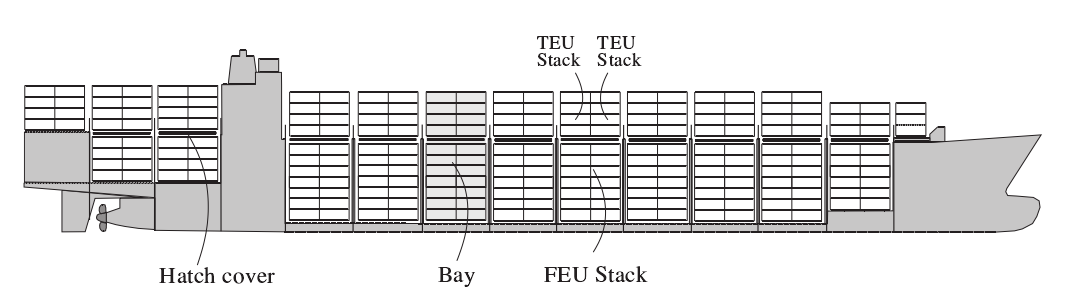
\includegraphics{figure/Arrangement_of_cargo_space.png}}
\caption{The arrangement of cargo space in a container vessel.}
\label{fig 1:graph}
\end{figure}

Each bay consists of container stacks placed along the width of the ship.
Stacks in a bay are indexed by a row number.
The position for one 20-ft container on the ship is uniquely indexed by (bay, row, tier), called a slot.
In addition, for some ships, two contiguous 20-ft bays form a 40-ft bay which can be used to accommodate 40-ft containers.

A ship usually calls a sequence of ports and containers are loaded and unloaded at each port by cranes in a last-in-last-out (LIFO) manner.
Rehandles arise either when we want to unload containers destined for the current port which however are beneath those destined for subsequent ports, or when we want to reorder the sequence of containers to prevent more rehandles in the future.
Rehandles are expensive, since on one hand terminals directly charge the carriers for such operations, on the other hand, rehandles make ships dwell at terminals longer, inducing more berthing cost.

Actual examples show that containership stowage plans not only influence the income of shipping company from transportation but also have a direct relation to the safety of ships and freights.
The problems have troubled and aroused the interests of both scholars and commercial shipping organization in many countries since 1970s~\citep{webster1970container}.
Most of the previous research on stowage planning focus on how to minimize the number of rehandles \citep{ding2015stowage,zhang2016multiobjective,zehendner2017algorithm}.

In this paper, we investigate the problem from a new perspective. We deal with Stowage Stack Minimization Problem (SSMP) which minimizes the number of used stacks.
The problem is of practical significance. In the real world, a carrier/forwarder may collect a few containers in a time interval and want to evaluate needed space (stacks), in order to estimate available space left.
Or on the contrary, a carrier/forwarder wants to receive provisional shipment orders as many as possible while reserving enough space for regular shipment orders.
Our algorithm provides them an indicator to achieve such goals.

The contribution of our paper lies in three aspects.
First, to the best of our knowledge, our paper considers the number of stacks used for the first time, and this is a very practical consideration.
As talked before, previous research usually focuses on how to reduce the rehandles or shifts.
Second, we analyze SSMP and give upper and lower bounds of SSMP. The bounds pave a way for future study.
Third, we propose a heuristic algorithm to solve SSMP and the algorithm has a performance guarantee.

The remainder of this paper is organized as follows: we review extant research works in Section~\ref{sec:lr}. The formal definition of SSMP and its properties are provided in Section~\ref{sec:pd}.
In Section~\ref{sec:algo}, we present our heuristic algorithm and the performance analysis.
Experiments are illustrated in Section~\ref{sec:ea}. Concluding remarks close the paper in Section~\ref{sec:con}.

\section{Literature review}
\label{sec:lr}
Based on the container handling locations occurred, the container handling problems can be divided into two streams; one is container management at terminals, and the other is containership stowage planning problems (CSP).
The problem discussed in this paper belongs to the latter.

Simulation methods based on probability, expert systems, decision support systems were mainly used in the early stages of the research.
\cite{webster1970container} first tried to solve the problem by using simulation methods with the help of computer.
\cite{shields1984containership} introduced a computer preplanning system (CAPS) which had been used by American President Lines.
The CAPS produced stowage plans by using Monte Carlo theory.
\cite{dillingham1986application} introduced their researches on expert system of stowage based on rules.
Each of the suggested container movements was displayed graphically as the decisions were made.
\cite{wilson2001container} outlined a computer system that generated good sub-optimal solutions to the stowage pre-planning problem.
The methodology progressively refined the arrangement of containers within the cargo-space of a container ship until each container is specifically allocated to a stowage location.

Most existing methods for the CSP are mathematical programming approaches.
\cite{botter1991stowage} created a mathematical model for the stowage plan problem, which used binary decision variables to determine the containers unloading and loading sequence for each port.
A 0-1 binary linear programming formulation was presented in order to minimize the number of shifts in \cite{avriel1998stowage} and \cite{avriel2000container}.
\cite{haghani2001model} proposed a MIP model for developing loading plans in order to minimize the time that a vessel spent at each port, and the container handling cost which shifts caused by was highly influenced by the number of unproductive but necessary an unsatisfactory arrangement of containers.
In \cite{ambrosino2004stowing}, the problem of stowing containers into a container ship had been faced by evaluating an exact 0-1 Linear Programming model, which was not practically useful for large cases.
\cite{ambrosino2015mip} proposed a Mixed  Integer  Programming (MIP) heuristic aimed at determining stowage plans in circular routes for container ships so as to give support for the ship coordinator and the terminal planner.
In \cite{parreno2016grasp}, they focused on the slot planning phase and presented a Constraint Programming and Integer Programming model for stowing a set of containers in a single bay section.

Apart from mathematical programming approaches, heuristic algorithms are also widely used in the research of CSP.
Three heuristic rules were used to assign gradually each type of containers to slots of the ship by four steps in \cite{scott1978loading}, while the shifting problem had not been considered in their model.
Tabu search was employed to obtain an optimal solution in \cite{wilson2001container}, \cite{bortfeldt2003parallel} and \cite{monaco2014terminal}.
\cite{ding2015stowage} developed a heuristic algorithm which can generate stowage plans with a reasonable number of shifts for such problems.
The algorithm, verified by extensive computational experimentations, performed better than the Suspensory Heuristic Procedure (SH algorithm) in \cite{avriel1998stowage}, which was a dynamic slot-assignment scheme.
The presented hybrid GA for loading a single container in \cite{bortfeldt2001hybrid} was particularly suitable for strongly heterogeneous containers stowage problems.
\cite{dubrovsky2002genetic}  used a GA for solving the stowage planning problem of minimizing the number of container movements.
Search space was significantly reduced by a compact and efficient encoding scheme.
The variant tackled in \cite{cohen2017container} involved several constraints, inspired by real-life problems and application found in the literature.

We have also read literature about container stowage problem with rehandles constraint.
\cite{malucelli2008stack} investigated stack reordering strategies aiming at minimizing the number of loading and unloading operations.
The complexity of stowage planning problem is investigated in \cite{tierney2014complexity} and it showed that the capacitated k-shift problem is solvable in polynomial time for any choice of stacks and stacks capacities.
A multi-objective ship stowage planning problem was researched by \cite{zhang2016multiobjective} and it aimed to optimize the ship stability and the number of rehandles simultaneously.

To the best of our knowledge, only \cite{avriel2000container} and \cite{jensen2010complexity} discussed the stowage stack minimization and its connection with the chromatic number of circle graphs when the stack height is unlimited apart from the SSMP-ZR researched by \cite{wang2014stowage}.


\section{Problem description and properties}
\label{sec:pd}
\subsection{Problem description and notation}
We put forward SSMP in this subsection.
Literally speaking, SSMP is a variant of CSP.
A ship starts its journey at port 1 and sequentially visits port 2, 3, ..., $P$. We assume the ship stops at port $P$.
$N$ containers are shipped along the journey.
At each port, the containers destined to the current port are discharged, and the containers await on yard are loaded to the ship.
We use $O(c)$ and $D(c)$ to denote the original and destination ports of container $c$, respectively. Accordingly, the itinerary is represented by a tuple $\{O(c), D(c)\}$.
Given $N$ containers to be shipped, the objective of SSMP is to figure out a stowage planning so as to minimize needed stacks.

If two containers $c1$ and $c2$ satisfy $O(c1)<O(c2)<D(c1)<D(c2)$, and $c2$ is placed above $c1$, then one \textit{rehandle} occurs, as we have to move $c2$ to the yard temporally for retrieving $c1$. Besides, containers above $c2$ also have to be moved, and therefore also extra rehandles occur.
In this paper, we extend SSMP with zero rehandle constraint in \cite{wang2014stowage}, assuming that $K$ rehandles are allowed.

Other assumptions assumed in this paper:
\begin{itemize}
\item Containers loaded are uniform standard 20-ft containers;
\item The information of $N$ containers are known in advance;
\item The containership is large enough to accommodate all the given containers;
\item Each stack can hold at most $H$ vertically piled containers, i.e., the height limit of every stack is $H$;
\item The balance of the containership can be resolved by assigning container stacks and water-ballast; hence, the balance is not considered when minimizing container stacks.
\end{itemize}

If the number of containers in a non-empty stack is less than $H$, the stack is termed as a \textit{partial} stack; otherwise it is a \textit{full} stack.
If rehandle occurs, containers above are called \textit{blocking containers} and the to-be-retrieved container is called \textit{target container}.
When moving blocking containers back to the ship, there is no guarantee that they will be returned to their original slots.

A feasible solution to the SSMP is represented by a sequence of operations. Each operation indicates the sequence number of container and its accommodating stack. Especially, the yard is term as stack 0. Moving a container $c$ to stack 0 means that $c$ is a blocking container and moved temporally on the yard.

\subsection{Integer model}
For the special case with zero rehandle, we only need to consider the loading process. For the unloading process, containers can be discharged in order without rehandles. The following IP model decides the accommodating stack of each container.
\begin{small}
\begin{align}
& (IP)~~\min\hspace{6pt}\sum_{s=1}^{S} y_s\notag\\
& \mathrm{s.t.}\hspace{11pt}\sum_{s=1}^{S} x_{is}=1, ~\forall 1\le i \le N \label{eqn:1}\\
%\mbox{s.t.~}& \sum_{c=1}^{C} x_{ic}=1, ~\forall 1\le i \le m \label{eqn:1}\\
& \hspace{24pt}\sum_{i=1}^{N} x_{is}\le M y_s, ~\forall 1\le s \le S	\label{eqn:2}\\
& \hspace{2pt}\sum_{i:O(i)\le p\le D(i)-1} x_{is}\le H, ~\forall 1\le s\le S, 1\le p\le P		\label{eqn:3}\\
& x_{is}+x_{js}\le 1, ~\forall 1\le s\le S, 1\le i,j\le N, O(j)<O(i)<D(j)<D(i)	\label{eqn:4}\\
& x_{is}, y_s \in \{0,1\}, ~\forall 1\le s\le S,1\le i,j\le N
\end{align}
\end{small}

In the above model, $M$ is a sufficiently large number and $S$ is the number of stacks on the ship.
$x_{is}$ is a binary decision variable which is equal to 1 if container $i$ is loaded to stack $s$, and 0 otherwise.
$y_s$ is a binary decision variable that is equal to 1 if stack $s$ is used for stowage, and 0 otherwise.
$O(i)$ and $D(i)$ indicate the shipping leg of container $i$.
The objective minimizes the number of stacks used.
Constraints (\ref{eqn:1}) ensure that each container $i$ is loaded to only one stack.
Constraints (\ref{eqn:2}) guarantee that containers can only be loaded to used stacks.
Constraints (\ref{eqn:3}) assure that at each port $p$, the number of containers in stack $s$ does not exceed $H$.
Constraints (\ref{eqn:4}) avoid rehandle requiring that container $i$ is prohibited to block container $j$ in the same stack when $O(j)<O(i)<D(j)<D(i)$.

The IP solution can be converted into a complete loading plan: start from port $p=1$ to port $p=P$. At port $p$, containers are sorted in a descending order of destination ports. Each container $i$ is loaded to the top of its corresponding stack $s^*$ which satisfies $x_{is^*}=1$.

For the IP model of general SSMP, it is hard to build a model.
Since there are rehandles, we have to move blocking containers in the yard and back to the ship.
The stacks of blocking containers are not necessarily the original slots.
If we want to model the slots of blocking containers, we have to set the variable $x_{ctl}$ that indicates the slot $t$ of a container $c$ at a layout $l$.
We do not know which containers are blocking containers in advance, therefore the domain of $c$ is the whole set of $N$ containers.
Especially, whenever we load or discharge a container, it forms a layout.
In addition, we do not know the number of layouts in advance.
All in all, the number of slots, containers, and layouts are numerous. Apart from other variables and constraints, the number of variable $x_{ctl}$ alone is too large to make the model meaningful and solvable.

\section{Methodology}
\label{sec:algo}
In this section, we will talk about the heuristic algorithm to solve the SSMP as well as the performance guarantee of the algorithm.

\subsection{Heuristic algorithm for the SSMP}
\label{sec:h1}
We first give some related notations for ease of exposition.

\begin{itemize}
\item $K$ means the number of allowed rehandles given in our problem.
\item $k$ means the number of real rehandles and it ranges from zero to $K$.
\item $nearport_s$ represents the value of the nearest port of stack $s$.
\item $NumofStack_p$ is referred as the largest number of used stacks after the ship's departure from port $p$.
\end{itemize}

Here is a simple example to illustrate $nearport_s$. Three containers are stored in stack $s$, and their destination ports are 4, 5, 6, respectively, then the value of $nearport_s$ is 4.
In particular, the value of $nearport_s$ of every empty stack $s$ is set as $P+1$.

Algorithm \ref{alg:1} solves instances of SSMP.

\begin{algorithm}[htbp]
  \caption{A heuristic procedure for the SSMP}
  \label{alg:1}
  \begin{codebox}
  \Procname{\proc{Heuristic(I)}}

    \li \For each port $p=1, 2 , \ldots,P $
    \li \Do
                Unload containers with $D(c)==p$.
    \li         Sort containers with $O(c)==p$ by the decreasing order of their destinations.
    \li         \For each container $c$ with $O(c)==p$
    \li         \Do
                   \If $k==K$
    \li            \Then
                        execute method $loading\_equalK(c)$.
    \li            \Else If $k < K$
    \li                 execute method $loading\_lessK(c)$.
                   \End
                \End
    \li          figure out the value of $NumofStack_p$.
        \End
    \li Output the value of $NumofStack_P$ in instance I.

 \end{codebox}
 \end{algorithm}

The main two stages in our heuristic algorithm are unloading and loading procedures.
Given an instance I, for each port $p$ along the voyage, containers with $D(c)==p$ are discharged one by one firstly.
Especially, if there exist blocking containers, they are moved on the yard temporally and regarded as containers to be loaded at the current port.
After containers with $D(c)==p$ are discharged, containers in the yard (including containers with $O(c)==p$ and blocking containers) are sorted in order and loaded.

At the end of our algorithm, the value of $NumofStack_P$ is given as an output after all the containers are processed at port $P$.

\subsection{Detail description of loading procedure}
\label{sec:d2}

Two different methods based on our greedy rules are adopted to choose stack for each loading container according to the relationship between $k$ and $K$ when loading containers at each port.
They are called as $loading\_lessK(c)$ and $loading\_equalK(c)$, respectively.
The detail description of the two loading methods will be introduced in this section.

We firstly talk about the simple condition that the allowed rehandles run out, i.e. $k==K$.
In the $loading\_equalK(c)$ method, we first consider choosing a stack from partial stacks with $nearport_s \ge D(c)$ for the loading container $c$.
If there are no such partial stacks exist, then one empty stack is necessary.
Therefore, the stack selection priority for container $c$ under this condition is:

\begin{enumerate}
\item the set of partial stacks, each stack $s$ in which satisfies the constraint that $nearport_s \ge D(c)$.
\item the set of empty stacks.
\end{enumerate}

%As mentioned above, the value of $nearport$ of every empty stack is set as $P+1$, the two kinds of stacks both meet the condition that their value of $nearport$ is no less than $D(c)$.
%Therefore, we add all the two kinds of stacks into the same $arraylist$ called $S_0$.
%For all the stacks in $S_0$, we choose the one with the smallest value of $nearport$.
%If there isn't one stack with the smallest value of $nearport$, we choose the first one when we traverse stacks in $S_0$.

Afterwards, we talk about the complex condition that some rehandles are allowed, i.e. $k < K$.
In the $loading\_lessK(c)$ method, the kinds of feasible stacks increase as a result of the existence of rehandles.
Under this condition, the stack selection priority for container $c$ becomes:

\begin{enumerate}
\item the set of partial stacks, which is indexed as $S_1$, each stack $s$ in $S_1$ meets the constraint that $nearport_s \ge D(c)$.
\item the set of partial stacks, which is indexed as $S_2$, each stack $s$ in $S_2$ meets the constraint that $nearport_s < D(c)$.
\item the set of empty stacks, which is indexed as $S_3$.
\end{enumerate}

Both in method $loading\_equalK(c)$ and $loading\_lessK(c)$, we need to clear all sets of stacks once we have chosen a stack for each loading container at every port.
Of course, we will update the value of $k$ if there is a rehandle when loading containers.
After loading the current container into the chosen stack $s*$, the height of $s*$ and $nearport_s*$ should both be updated.

Actually, a lot of variables and methods of the specific unloading and loading strategies have been involved, we do not write all of them here for the sake of context length.
For example, the method to record the information of loading and unloading operations is not given in this paper.

It's worth mentioning that our algorithm can figure out the detailed location changes of each container and output the layout status in the containership at an arbitrary time.
In other words, we can predict the real-time container stowage process before the voyage as long as we know some information in advance.
Therefore, our algorithm makes difference and makes some sense in the real application.


\subsection{Performance Guarantee of the Algorithms}
\label{sec:p3}

In order to show that the heuristic algorithms have a performance guarantee, we prove the bounds of feasible solutions to the problem.
For ease of exposition, we first give some related notations.

\begin{itemize}
\item $\mathcal{C}^*$: the optimal solution to the SSMP instances.
\item $\mathcal{C}$: the solution to the SSMP instances by the algorithm.
\item $N_p$: the number of containers on the ship before its departure from port $p$.
\item $V_p$: the number of loading ports that the ship has visited before it departs from port $p$.
\end{itemize}

It should be noted that a port is called a loading port if there exists at least one container to be loaded. Clearly, $V_p \le p$, $\forall p=1,\ldots,P$.

\begin{proposition}
The SSMP instance has a lower bound:
\begin{equation*}
\max\limits_{p=1,\ldots,P}(\lceil\frac{N_p}{H}\rceil) \le \mathcal C^*
\end{equation*}
\label{pro:a1}
\end{proposition}

\begin{proof}

$\lceil\frac{N_p}{H}\rceil$ is the least number of stacks to accommodate all the containers at port $p$, and thus, $\max\limits_p(\lceil\frac{N_p}{H}\rceil)$ is the least number of stacks needed throughout the journey.
\end{proof}

The lower bound can be a reference to check the optimality of solutions obtained by our heuristic.
We can conclude that the solution is close to optimal if the solution is close to the lower bound.

In order to facilitate the solution, we divide the stack used in the port into two parts: full stacks and partial stacks.
For the full stacks, the number of full stacks in port $p$ is no greater than $\lfloor\frac{N_p}{H}\rfloor$, which is easy to be proven.
For the partial stacks, we define the number of partial stacks in port $p$ as $P(p)$, and we have Proposition \ref{pro:a2} for $P(p)$.
\begin{proposition}
The number of partial stacks in port $p$ is no greater than $V_p$:
\begin{equation*}
 P(p) \le  V_p
\end{equation*}
\label{pro:a2}
\end{proposition}

\begin{proof}

To get this proposition proven, we divide the stacks into different partitions to store containers according to the number of loading ports.
Actually, the number of partitions is equal to the number of loading ports.
A new partition will be assigned when the ship arrives at a loading port.

In every partition, there will be no rehandles since all containers at each port is sorted in order before being loaded.
If it is not a loading port, there is no need to divide a new partition and the number of partial stacks will not change.
If it is a loading port and the number of containers to be loaded happens to be an integer multiple of limited height $H$, then the number of partial stacks in the new partition is zero.
Otherwise, a new partial stack will be produced in the new partition.
Therefore, the number of partial stacks in a new partition during the loading process is no greater than one at every port.

Similarly, the number of partial stacks in each partition is still no greater than one after discharging containers.
If there are not containers to be discharged at the current port, the number of partial stacks in each partition is the same as the former port.
Otherwise, the number of partial stacks in each partition will convert between zero and one or stay unchanged.
In a word, the number of partial stacks in each partition is one at most and thus the total number of partial stacks after the unloading process is no greater than the number of partitions, i.e. the number of loading ports.

We use an inductive proof.

\textit{Basis}: For $p=1$, without loss of generality, we assume that port 1 is a loading port, and therefore $V_1$ =1.
In addition, P(1)=0 or 1, i.e. $P(1) \le 1$. Hence, $P(p) \le V_p $ holds.

\textit{Inductive step}: Suppose that the partial stacks in port $i$ is no greater than $V_i$, i.e. $P(i) \le V_i $.
Upon the ship arrives at port $i+1$, it first unloads containers with $D(c)=i+1$ at each partition.
After unloading containers with $D(c)=i+1$, the number of partial stacks at all the partitions is still at most $V_i$, the number of loading ports.

(1) If there are containers to be loaded at port $i+1$, they will be loaded into the new partition for $p=i+1$ and there will be at most one more partial stacks to be produced, then $V_{i+1}=V_i+1$,  $P($i+1$) \le P(i)+1$. Hence, $P($i+1$) \le P(i)+1 \le V_i+1=V_{i+1}$

(2) If there is no containers to be loaded at port $i+1$,  $V_{i+1}=V_i$, $P($i+1$) \le V_i$. Hence, $P($i+1$) \le V_{i}=V_{i+1}$.

Based on the above two steps, we have $P(p) \le V_p,  \forall p=1,\ldots,P$.
\end{proof}


\begin{proposition}
For the heuristic solution to the SSMP instance, it holds
\begin{equation*}
\mathcal{C}^* \le \mathcal{C} \le \max_{p=1,\ldots,P}(\lfloor\frac{N_p}{H}\rfloor+V_p) \le \mathcal{C}^*+V_P
\end{equation*}
\label{pro:a3}
\end{proposition}

\begin{proof}

The first inequality obviously holds.

For the second inequality, $\mathcal{C}=\max\limits_p \mathcal{C}_p$.
Noted that $\mathcal{C}_p$ is the number of used stacks in port $p$ obtained from our algorithm and it includes the number of full stacks and the number of partial stacks.
As the number of full stacks in port $p$ is no greater than $\lfloor\frac{N_p}{H}\rfloor$ and the number of partial stacks in port $p$ is no greater than $V_p$.
Therefore, the second inequality holds.
For the third inequality, $\lfloor\frac{N_p}{H}\rfloor\leq \lceil\frac{N_p}{H}\rceil$, and $\lceil\frac{N_p}{H}\rceil$ is the lower bound of the number of stacks used at port $p$ by Proposition \ref{pro:a1}.
Thus, $\lfloor\frac{N_p}{H}\rfloor \le \mathcal{C}_p^*$.
It then holds $\max\limits_p(\lfloor\frac{N_p}{H}\rfloor+V_p) \le \max\limits_p(\mathcal{C}^*+V_p) = \mathcal{C}^*+V_P$.
\end{proof}


The above propositions show that our heuristic algorithm has a constant performance guarantee.
In the real shipping transportation, the number of ports is generally much smaller than the number of used stacks.
Therefore, the difference between the optimal solution and our heuristic solution is relatively small, which indicates that our heuristic algorithms can generate promising solutions.


\section{Experiments and Analysis}
\label{sec:ea}

This paper uses the test data from \cite{wang2014stowage} and we add an extra parameter $K$ into the previous instances in order to meet the demands of research.
$K$ means the number of allowed rehandles here and it has a significate influence on our research problem.
Particularly, we regard instances with $K=0$ as the benchmark instances comparing with the same instances with different values of $K$.
In fact, the problem becomes SSMP-ZR when $K=0$.
There are 360 sets of instances, or 1800 instances in total, which are categorized by four parameters: the number of allowed rehandles, which is selected from \{0, 10, 20, 50, 100\};
the number of ports $P$, which is selected from \{5, 10, 20, 30\};
the number of containers $N$, which is selected from \{50, 100, 200, 500, 1000, 5000\};
and the height limit $H$, selected from \{4, 8, 12\}.
Each set consists of 5 instances generated by different random seeds.
In each instance, the origin $O(i)$ and the destination $D(i)$ of a container $i$ are generated from a uniform distribution on the integers $1, 2, \ldots, P$ satisfying that $O(i)<D(i)$.
For the convenience of comparison, we only show the average value of $Numofstack_P$ when $K=0$, $K=10$, $K=20$, $K=50$, $K=100$, respectively.

In this section, we will showcase the performance of our heuristic algorithms on a number of test instances.
The heuristic was implemented in Java and the experiments were conducted on a computer with Intel Core processor clocked at 2.30 GHz and 8 GB RAM.
The operating system of the computer is Windows 10.

The experimental results are shown in Table \ref{tab:2} and Table \ref{tab:3}.
Considering the size of the table, the results of instances with $N=5000$ are not listed.

\begin{table}[htbp]
\footnotesize
  \centering
  \setlength{\belowcaptionskip}{10pt}
  \caption{Results of the instances with $P\in\{5, 10\}$}
  \begin{tabular}{ccccccccccccccc}
  \hline
  \multicolumn{1}{c}{\multirow{2}{*}{P}}
  & \multicolumn{1}{c}{\multirow{2}{*}{N}}
  & \multicolumn{1}{c}{\multirow{2}{*}{H}}
  & \multicolumn{7}{c}{Heu}
  & \multicolumn{5}{c}{Ran}\\
  \cline{4-15}
  \multicolumn{1}{c}{}
  &\multicolumn{1}{c}{}
  &\multicolumn{1}{c}{}
  &\multicolumn{1}{c}{LB}&{UB}&{K=0}&{K=10}&{K=20}&{K=50}&{K=100}
  &\multicolumn{1}{c}{K=0}&{K=10}&{K=20}&{K=50}&{K=100}\\
  \hline

    5     & 50    & 4     & 8     & 9.6   & 8     & 8     & 8     & 8     & 8     & 12.2  & 9.6   & 10.4  & 9.6   & 9.6 \\
    5     & 50    & 8     & 4     & 6     & 4.6   & 4     & 4     & 4     & 4     & 10    & 8.4   & 8     & 9.6   & 7.8 \\
    5     & 50    & 12    & 3     & 5     & 3.2   & 3.2   & 3     & 3     & 3     & 9.2   & 9.2   & 7     & 8.6   & 7.6 \\
    5     & 100   & 4     & 15    & 16.8  & 15    & 15    & 15    & 15    & 15    & 18.4  & 16.2  & 16.2  & 16.6  & 16.6 \\
    5     & 100   & 8     & 7.6   & 9.6   & 7.6   & 7.6   & 7.6   & 7.6   & 7.6   & 14.2  & 14.8  & 12.8  & 12    & 13.2 \\
    5     & 100   & 12    & 5.4   & 7.6   & 5.4   & 5.6   & 5.4   & 5.4   & 5.4   & 14.2  & 14.4  & 12.6  & 13.2  & 12 \\
    5     & 200   & 4     & 30.6  & 32.2  & 30.6  & 30.6  & 30.6  & 30.6  & 30.6  & 32.8  & 32.4  & 32.4  & 32    & 33 \\
    5     & 200   & 8     & 15.6  & 17.4  & 15.6  & 15.6  & 15.6  & 15.6  & 15.6  & 23.6  & 24.6  & 22.4  & 19.4  & 20.4 \\
    5     & 200   & 12    & 10.4  & 12.4  & 10.4  & 10.4  & 10.4  & 10.4  & 10.4  & 21.8  & 22.8  & 20.4  & 19.2  & 16.2 \\
    5     & 500   & 4     & 76.6  & 78    & 76.6  & 76.6  & 76.6  & 76.6  & 76.6  & 78.6  & 78.6  & 78    & 77.8  & 79 \\
    5     & 500   & 8     & 38.6  & 40    & 38.6  & 38.6  & 38.6  & 38.6  & 38.6  & 46    & 44.4  & 45    & 42.8  & 42 \\
    5     & 500   & 12    & 26    & 27.4  & 26    & 26    & 26    & 26    & 26    & 38    & 36.2  & 39.8  & 37.6  & 33.8 \\
    5     & 1000  & 4     & 152.2 & 153.8 & 152.2 & 152.2 & 152.2 & 152.2 & 152.2 & 153.6 & 153.6 & 154.2 & 154.2 & 153.4 \\
    5     & 1000  & 8     & 76.6  & 78.2  & 76.6  & 76.6  & 76.6  & 76.6  & 76.6  & 82.2  & 81.8  & 81.4  & 80.2  & 79.6 \\
    5     & 1000  & 12    & 51    & 52.8  & 51    & 51    & 51    & 51    & 51    & 61.4  & 60.8  & 60.4  & 63    & 60.4 \\
    10    & 50    & 4     & 7.8   & 12.6  & 9     & 8     & 7.8   & 7.8   & 7.8   & 12.4  & 11    & 10.2  & 9.8   & 9.6 \\
    10    & 50    & 8     & 4     & 10    & 6     & 6     & 5     & 4     & 4     & 10.8  & 10.8  & 10.4  & 8.8   & 8.8 \\
    10    & 50    & 12    & 3     & 9.4   & 5.6   & 4.6   & 4.4   & 3.2   & 3     & 12    & 11.4  & 9     & 8.8   & 8.6 \\
    10    & 100   & 4     & 14.8  & 19.6  & 15.8  & 15.6  & 15    & 14.8  & 14.8  & 20.4  & 20.2  & 20.2  & 16.8  & 17.4 \\
    10    & 100   & 8     & 7.6   & 12.6  & 9.2   & 9.8   & 9.6   & 7.8   & 7.6   & 20    & 18.4  & 17    & 13.6  & 13.6 \\
    10    & 100   & 12    & 5.2   & 10.4  & 7     & 7     & 7.2   & 6.4   & 5.2   & 18.4  & 17.8  & 17.6  & 13.8  & 14.2 \\
    10    & 200   & 4     & 28.6  & 33.2  & 29.6  & 29.6  & 28.6  & 28.6  & 28.6  & 35.4  & 36    & 34.4  & 31.4  & 30.6 \\
    10    & 200   & 8     & 14.4  & 19.2  & 16.4  & 16.6  & 16.2  & 14.8  & 14.4  & 28.6  & 29.2  & 25.6  & 27.4  & 23 \\
    10    & 200   & 12    & 9.8   & 15    & 12    & 12    & 11.8  & 11.4  & 9.8   & 26.4  & 27.2  & 26.8  & 24.2  & 24 \\
    10    & 500   & 4     & 69.8  & 74.2  & 69.8  & 69.8  & 69.8  & 69.8  & 69.8  & 78    & 75.4  & 74.6  & 74.2  & 71.2 \\
    10    & 500   & 8     & 35    & 39.4  & 35.6  & 35    & 35.2  & 35    & 35    & 52.8  & 49.4  & 52.6  & 51.4  & 52.6 \\
    10    & 500   & 12    & 23.6  & 28    & 25.2  & 24.8  & 24.8  & 24    & 23.6  & 50.2  & 48.4  & 50    & 47.4  & 47.6 \\
    10    & 1000  & 4     & 137.6 & 141.8 & 137.6 & 137.6 & 137.6 & 137.6 & 137.6 & 143.2 & 143.8 & 143.4 & 141.8 & 140.2 \\
    10    & 1000  & 8     & 69    & 73.2  & 69.2  & 69    & 69.2  & 69    & 69    & 87.8  & 84.8  & 85.8  & 86    & 85.2 \\
    10    & 1000  & 12    & 46.2  & 50.4  & 46.6  & 46.8  & 46.8  & 46.6  & 46.2  & 77.2  & 78    & 74.4  & 76.4  & 74.8 \\

    \hline
    \end{tabular}
  \label{tab:2}
\end{table}


\begin{table}[htbp]
\footnotesize
  \centering
  \setlength{\belowcaptionskip}{10pt}
  \caption{Results of the instances with $P\in\{20, 30\}$}
  \begin{tabular}{ccccccccccccccc}
  \hline
  \multicolumn{1}{c}{\multirow{2}{*}{P}}
  & \multicolumn{1}{c}{\multirow{2}{*}{N}}
  & \multicolumn{1}{c}{\multirow{2}{*}{H}}
  & \multicolumn{7}{c}{Heu}
  & \multicolumn{5}{c}{Ran}\\
  \cline{4-15}
  \multicolumn{1}{c}{}
  &\multicolumn{1}{c}{}
  &\multicolumn{1}{c}{}
  &\multicolumn{1}{c}{LB}&{UB}&{K=0}&{K=10}&{K=20}&{K=50}&{K=100}
  &\multicolumn{1}{c}{K=0}&{K=10}&{K=20}&{K=50}&{K=100}\\
  \hline

    20    & 50    & 4     & 7.2   & 19.6  & 9     & 9     & 8     & 7.2   & 7.2   & 13    & 12.2  & 10.8  & 10.2  & 9.6 \\
    20    & 50    & 8     & 3.8   & 19    & 7.8   & 7     & 6.6   & 5.4   & 3.8   & 12.8  & 13    & 10.8  & 8.8   & 8.8 \\
    20    & 50    & 12    & 2.8   & 19    & 7.8   & 6.6   & 5.6   & 4     & 2.8   & 13.6  & 12.4  & 11    & 8     & 8 \\
    20    & 100   & 4     & 14.2  & 25    & 16    & 16    & 16    & 14.2  & 14.2  & 21    & 21.8  & 22.2  & 17.8  & 16 \\
    20    & 100   & 8     & 7.4   & 19.6  & 10.8  & 11    & 10.8  & 10.2  & 7.6   & 20.6  & 19.4  & 19.4  & 17.4  & 13.4 \\
    20    & 100   & 12    & 5     & 19.2  & 10.2  & 9.8   & 9     & 9     & 7.6   & 21.2  & 21.4  & 20    & 18.4  & 13 \\
    20    & 200   & 4     & 27.6  & 37.6  & 29.8  & 30.2  & 29.8  & 28.8  & 27.6  & 39.6  & 37    & 37.2  & 36.4  & 31.8 \\
    20    & 200   & 8     & 14.2  & 25.2  & 17.6  & 18    & 18    & 17.4  & 17.4  & 33.4  & 35.4  & 32    & 31.8  & 28.6 \\
    20    & 200   & 12    & 9.4   & 21.6  & 13.8  & 13    & 13.8  & 13.2  & 13.4  & 33.8  & 31.6  & 31.8  & 30.2  & 30.8 \\
    20    & 500   & 4     & 67.6  & 77.2  & 70.2  & 70.4  & 70    & 70.4  & 67.6  & 80    & 81    & 80.8  & 80.4  & 77.8 \\
    20    & 500   & 8     & 34    & 43.6  & 38    & 37.6  & 37.8  & 38    & 38    & 64.2  & 64.6  & 62.6  & 61.4  & 61 \\
    20    & 500   & 12    & 22.8  & 33.2  & 27    & 27.2  & 27.2  & 27.2  & 27.2  & 60.8  & 61.6  & 62.4  & 59.8  & 58 \\
    20    & 1000  & 4     & 134.4 & 143.6 & 135.8 & 135.8 & 136.2 & 136   & 134.4 & 148   & 146   & 148.6 & 148.4 & 147.4 \\
    20    & 1000  & 8     & 67.6  & 76.8  & 70.6  & 71    & 70.4  & 70.4  & 70.6  & 102.2 & 101.6 & 101   & 100.2 & 100.8 \\
    20    & 1000  & 12    & 45.2  & 54.4  & 48.8  & 49.8  & 49.2  & 49.2  & 48.8  & 93.8  & 97.4  & 97.4  & 94.8  & 91.6 \\
    30    & 50    & 4     & 8     & 29.8  & 10    & 9.8   & 9.4   & 8     & 8     & 15.8  & 13.4  & 11    & 10.6  & 10.6 \\
    30    & 50    & 8     & 4.2   & 29    & 8.2   & 7.8   & 7.6   & 5.2   & 4.2   & 15.8  & 13.2  & 11.6  & 10    & 9.6 \\
    30    & 50    & 12    & 3     & 29    & 8     & 7.4   & 6.8   & 5.2   & 3.4   & 14.6  & 14.4  & 12.8  & 9     & 8.8 \\
    30    & 100   & 4     & 13.8  & 33.4  & 16.8  & 16.6  & 16.2  & 15.6  & 13.8  & 22.4  & 22.8  & 22.8  & 19.6  & 16.6 \\
    30    & 100   & 8     & 7.2   & 29.6  & 12    & 11.4  & 11.8  & 10.8  & 9.8   & 22    & 21.8  & 20.8  & 19    & 15 \\
    30    & 100   & 12    & 5     & 29    & 10.8  & 10.4  & 10.2  & 9.8   & 8.2   & 21.8  & 21.8  & 20.4  & 19.8  & 15.2 \\
    30    & 200   & 4     & 27.6  & 43.8  & 30.4  & 31    & 31.6  & 31.2  & 28    & 40.6  & 39.8  & 41.2  & 38.6  & 34 \\
    30    & 200   & 8     & 14    & 32.2  & 18.6  & 18.8  & 19    & 19.4  & 19.8  & 36.4  & 36.2  & 36.2  & 36.8  & 32.8 \\
    30    & 200   & 12    & 9.6   & 29.8  & 17    & 16.6  & 16.2  & 16.2  & 16.2  & 35.6  & 36    & 37    & 34.8  & 33.4 \\
    30    & 500   & 4     & 64.8  & 80.4  & 69.6  & 69.6  & 69.6  & 69.4  & 69.2  & 83.2  & 82.2  & 82.8  & 82    & 81.8 \\
    30    & 500   & 8     & 32.6  & 49    & 38.4  & 38.6  & 38.6  & 38.2  & 37.8  & 68.8  & 66    & 68.6  & 70.6  & 66.4 \\
    30    & 500   & 12    & 22.2  & 39.2  & 29    & 29    & 28.6  & 28.6  & 28.8  & 69.2  & 67.4  & 66.2  & 66.6  & 66 \\
    30    & 1000  & 4     & 128.8 & 144   & 133.6 & 133.6 & 133.6 & 133.8 & 133.6 & 149   & 150.8 & 150   & 147.8 & 150.6 \\
    30    & 1000  & 8     & 64.8  & 80.4  & 71.4  & 70.6  & 71    & 70.6  & 70.6  & 111.2 & 112.8 & 111.8 & 110.6 & 110 \\
    30    & 1000  & 12    & 43.2  & 59.4  & 50.8  & 50.6  & 50.8  & 50.8  & 50.8  & 107.6 & 108.8 & 108.6 & 107   & 101.2 \\

    \hline
    \end{tabular}
  \label{tab:3}
\end{table}

Table \ref{tab:2} summarizes the results of those easy instances with smaller number of ports, i.e. $P \in \{5, 10\}$.
For each given $P$, $N$ and $H$, we work out the values of $LB$, $UB$ of our heuristic algorithm.
For both our heuristic algorithm and random algorithm, we work out the average numbers of $Numofstack_P$ in different instances when $K$ is set to different values.
The $LB$ and $UB$ are used to test the rationality of heuristic algorithm and the average $Numofstack_P$ of instances with different values of $K$ by using heuristic and random algorithms are used to compare with each other.

Table \ref{tab:3} summarizes that the results of those difficult instances with larger number of ports, i.e. $P \in \{20, 30\}$.
The columns in Table \ref{tab:3} are similarly defined as those of Table \ref{tab:2} and so is the conclusion we can get from Table \ref{tab:2}.

Most of the instances provide the evidence that it works better when $K$ is not equal to zero comparing the condition where $K$ is equal to zero.
However, results between easy instances and difficult instances have some differences.
Comparing with the significant influence of different $K$ in the difficult instances, the influence of different $K$ in easy instances is not so obvious.
The same conclusion can be drawn if we focus on every single variable or factor while keeping other variables unchanged.

After a deep thinking and analysis, we found that it is the density and sparseness of stacks that causes this consequence.
In other words, the smaller value of each variable is, the same kind of containers with the identical origin port and destination port have more chance to be placed in the same stack and less rehandles will arise.
We call this kind of stack with high density, and high sparseness in contrast.

For each instance with the same $P$, $N$ and $H$, we call it benchmark instance when $K$ is equal to zero.
When $K$ is not equal to zero in an instance, we call it an exceptional instance if the number of used stacks is larger than the result of its benchmark instance.
There are few exceptions when we analyze the result through a large number of experiments.
Comparing with zero rehandle, the number of needed stacks is even larger when the number of allowed rehandle $K$ is not equal to zero, though the deviation is not great.

We then find out those exceptional instances and compare the stowage planning with the same instances under the zero rehandle constraint, and we find it is the distribution status of previous containers to be blamed.
In fact, the allowed rehandles delay the production of new stacks but not to reduce them, that is why the problem happens.
After all, it's the unloading strategy for blocking containers that causes this exceptional condition.
Because we reset the origin port of blocking containers, the loading containers in current port increase and meanwhile the allowed rehandles run out.
In the end, the extra and new stacks are needed under the coincidence.
In order to prove it, we output the layout of the exceptional instances and the corresponding benchmark instances.
By comparing the layout between exceptional instances and the corresponding benchmark instances, we get the conclusion that both the distribution of containers and the algorithm are blamed for this kind of abnormal condition.

However, it does not mean that our algorithm is inapplicable or our algorithm does not have a universality because the probability of causing exceptional instances is very low and it hardly happens in our practical operations.
Actually, our heuristics algorithm is feasible for most of the instances and has a good performance as well.
The following tables and figures can be used to illustrate the good performance of our algorithm.

We analyze the average result of all instances and some conclusions are drawn.
Table \ref{tab:4} and Figure \ref{fig 2:graph} give the average results of heuristic and random algorithm when the number of allowed rehandle $K$ is set to different values.
It's not difficult to draw the conclusion that the number of used stacks gets smaller as the allowed rehandle becomes larger for both heuristic algorithm and random algorithm.
Another conclusion is, comparing with the random algorithm, our heuristic algorithm has a fairly good performance to work out the solution.
It's noteworthy that the average results in Table \ref{tab:4} include the instances with $N=5000$.

\begin{table}[htbp]
  \centering
  \setlength{\belowcaptionskip}{10pt}
  \caption{average results of the instances with different K for two algorithms}
    \begin{tabular}{r|r|r|r|r|r}
    \hline
     $K$       &0   &10  &20  &50  &100\\
    \hline
    $Numofstack$ of Heu   &99.3  &99.21944  &99.08333   &98.73889  &98.35\\
 \hline
    $Numofstack$ of Ran  &114.62778  &114.31667  &114.21448  &112.86111 &111.9\\
 \hline
    \end{tabular}
  \label{tab:4}
\end{table}

\begin{figure}[htbp]
\centering
\setlength{\abovecaptionskip}{10pt}
\resizebox{1.0\textwidth}{!}{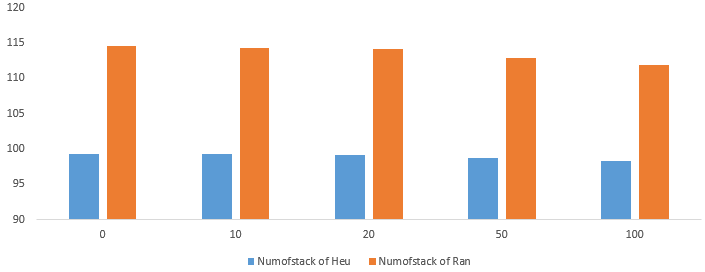
\includegraphics{figure/result_Heu&Ran.png}}
\caption{Numofstack of Heu and Ran with different K.}
\label{fig 2:graph}
\end{figure}

There is a simple illustration to elaborate why a certain number of allowed rehandles can improve the utilization of containership comparing with zero rehandle.
Assuming that there are thirteen containers to be transported along the voyage with six ports.
We let C($i$,$j$) denote index container whose origin port is $i$ and destination port $j$.
The following is the way to denote those containers: four containers are C(1,3), one is C(2,4), one is C(2,6), four are C(3,5), one is C(4,6) and two are C(5,6).

If they are loaded without any rehandles, the loading sequence and layout will be the following Figure \ref{fig 3:graph}.
\begin{figure}[htbp]
\centering
\setlength{\abovecaptionskip}{10pt}
\resizebox{1.0\textwidth}{!}{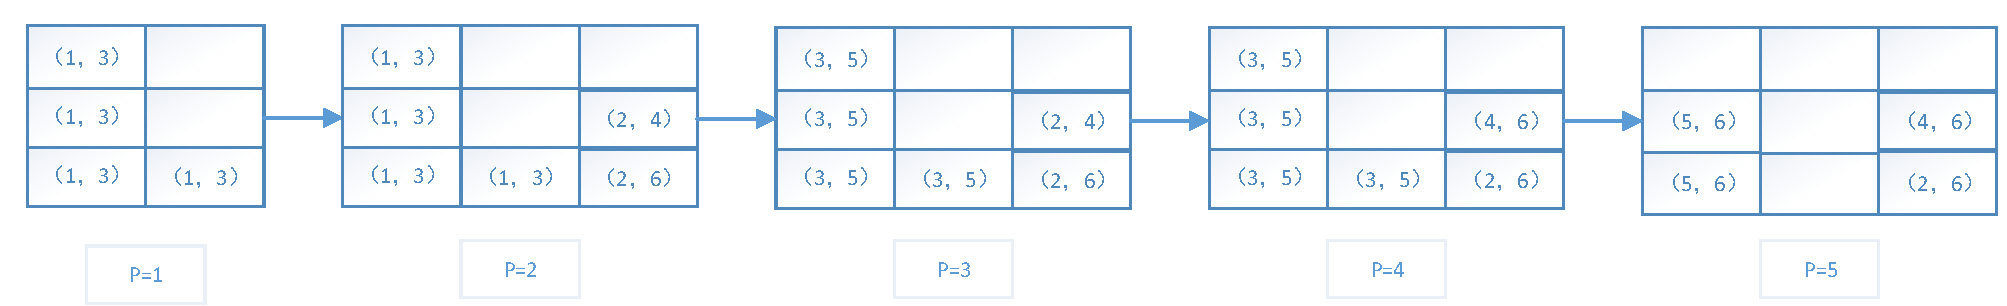
\includegraphics{figure/without_rehandle.jpg}}
\caption{stowage plan without rehandle.}
\label{fig 3:graph}
\end{figure}


If they are loaded with enough rehandles, the loading sequence and layout will be the following Figure \ref{fig 4:graph}.
\begin{figure}[htbp]
\centering
\setlength{\abovecaptionskip}{10pt}
\resizebox{0.9\textwidth}{!}{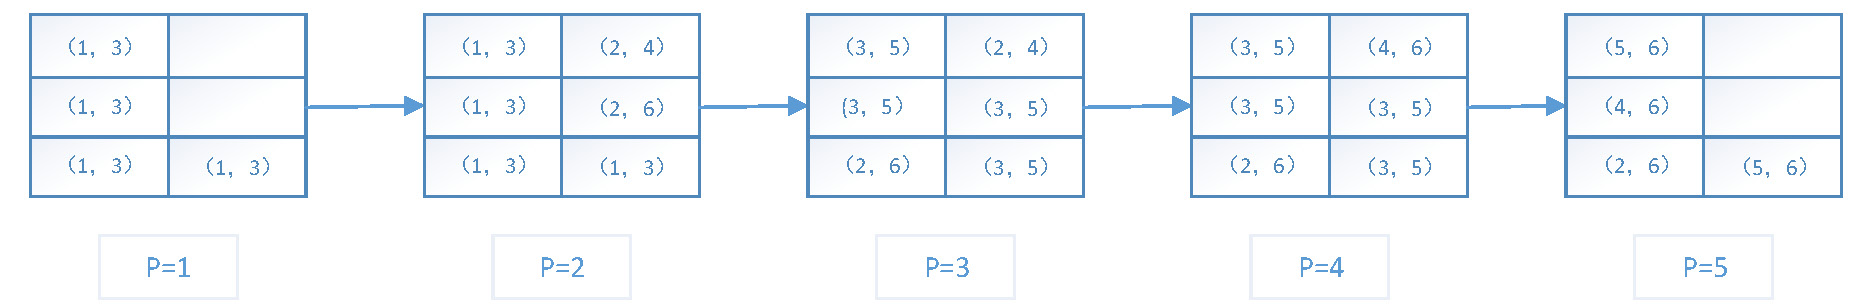
\includegraphics{figure/with_rehandle.jpg}}
\caption{stowage plan with rehandle.}
\label{fig 4:graph}
\end{figure}


From Figure \ref{fig 3:graph} and \ref{fig 4:graph}, we can clearly get the conclusion that allowing a certain number of rehandles will reduce the number of stacks used to store containers in a vessel compared with zero rehandle.
That's to say, the utilization of containership can be improved if some rehandles are allowed.

As a matter of fact, we have tried a related algorithm named $P\&H$ algorithm to get the optimal stowage planning before adopting our current heuristic algorithm.
This algorithm is actually a process of parameter tuning, our original intention is attempting to find out a better solution to stow containers.
Nevertheless, the result of this algorithm is not as good as the heuristic algorithm and it does not work well as we expected if the value of $K$ is small.
From another point of view, it just shows the good performance of our heuristic algorithm.

In our $P\&H$ algorithm, we give some restrictions on the height and the destination port of current loading container when choosing an optimal stack for current loading container.
Both the parameters in $P\&H$ value between 0 and 1, and zero is not included.
The former parameter represents the ratio of the $D(c)$ and the farthest port $P$, $c$ is the sequence number of current loading container.
The value of this parameter is 1 if $D(c)==P$.
The latter parameter represents the ratio of feasible stack's height and the limited height $H$.
The main idea of the $P\&H$ algorithm is to take the destination port of loading container and the limit height of stack into consideration when choosing the best stack for each loading container.
The purpose of this algorithm is to load those containers with farther destination port into the bottom of the stack and the computational result will be listed in the Table \ref{tab:5}.

\begin{table}[htbp]
  \centering
  \setlength{\belowcaptionskip}{10pt}
  \caption{average results of the instances with $P\&H$ algorithm}
    \begin{tabular}{r|r|r|r|r|r}
    \hline
     $P\&H$       &0   &10  &20  &50  &100\\
    \hline
    $0.75\&0.75$   &99.32222  &99.24167  &99.08056   &98.725  &98.29167\\
    \hline
    $0.75\&0.80$   &99.32222  &99.24167  &99.08056   &98.725  &98.29167\\
    \hline
    $0.80\&0.75$   &99.30833  &99.225  &99.05556   &98.71111  &98.31389\\
    \hline
    $0.80\&0.80$    &99.30833  &99.225  &99.05556   &98.71111  &98.31389\\
    %\hline
%    $1.0\&1.0$      &97.68542  &97.61042  &97.4875    &97.15  &96.77708\\
    \hline
    \end{tabular}
  \label{tab:5}
\end{table}

Table \ref{tab:5} shows the result with the $P\&H$ algorithm, which is firstly designed to improve the original algorithm and eventually it is used to prove the good performance of our original algorithm.
It's noteworthy that the average results in Table \ref{tab:5} include the instances with $N=5000$, too.
Both the values of two parameters in the $P\&H$ algorithm are selected form \{0.75, 0.8\}.
It's clear that the result shows the allowed rehandles will decrease the number of used stacks as the above results in Table \ref{tab:4}.
What's more, we can draw a conclusion that the first parameter has a significant influence on the result while the second parameter makes no difference if we compare the result in each row.

To find the relationship between the related variables and the results obtained from our heuristic, we make Figure \ref{fig 5:graph} using data from our results to facilitate us to find patterns.
$K$ is selected from \{0,100\}, $P$ is selected from \{5,30\}, $N$ is selected from \{50,200,1000\} and $H$ is selected from \{4,12\} in Figure \ref{fig 5:graph} so that we can find out the related relationships clearly.

\begin{figure}[htbp]
\centering
\setlength{\abovecaptionskip}{10pt}
\resizebox{0.9\textwidth}{!}{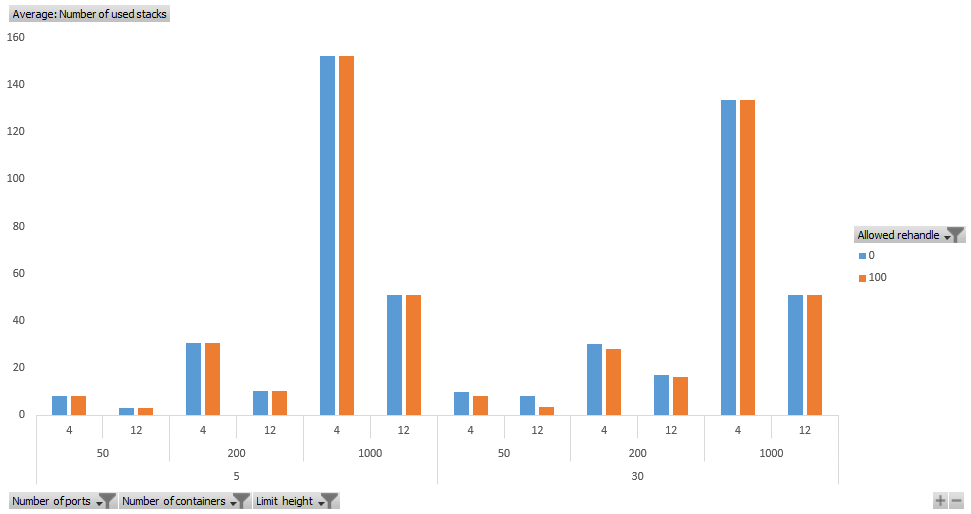
\includegraphics{figure/comprehensive_analysis.png}}
\caption{comprehensive analysis.}
\label{fig 5:graph}
\end{figure}

Observing from Figure \ref{fig 5:graph}, we can get the following relationships.
On one hand, the more ports, the more containers and the higher limited height will result in the more needed stacks whether we consider the influence of univariable or multivariable.
On the other hand, the difference in the results between zero rehandle and certain allowed rehandles becomes more and more obvious as the number of port gets larger, the limited height gets higher and the number of container gets smaller.

In short, the rationality and good performance of our heuristic have been confirmed by all the above tables and figures.

\section{Conclusion}
\label{sec:con}
The stowage stack minimization problem with K-rehandle constraint is aimed to find out a stowage plan that fewest stacks on a containership are required to accommodate given containers throughout a voyage by subject to K-rehandles.
Actually, the stowage stack minimization problem with zero rehandle is regarded as a particular case of SSMP when $K$ is set to zero.
The other way round, the problem proposed in this paper is a generalized and extended problem of SSMP-ZR considering the existence of $K$ rehandles.

In this paper, we first presented the integer programming model for the SSMP-ZR in \cite{wang2014stowage}.
However, it is hard to build an IP model for the stowage stack minimization problem with K-rehandle.
A heuristic approach is then proposed to construct solutions to the SSMP problem in a very short computational time.
The performance guarantee of our heuristic algorithm is proven with the solution of lower and upper bounds, which pave a way for future study.

The experimental results show that our heuristic approaches generate very promising solutions on a variety of instances.
Through experimental analysis, it can be found that it is meaningful to take the number of stacks used into consideration.
The results show the problem we put forward is of practical significance and it does reduce the number of stacks used and improve the utilization of containership.

The novelty and practicality show the importance of this paper and it can give a reference to the future study.
In the further research, more heuristic and precise algorithms will be used to find solutions to the stowage stack minimization problem.

%\section*{Acknowledgments}
%
%This research was partially supported by the National Natural Science Foundation of China [grant number 71602109]; Shanghai Pujiang Program [grant number 16PJC038]; and Funding Program for Teachers of Shanghai High Education [grant number ZZSD15095].

\bibliographystyle{apalike2}
\bibliography{references}

\end{document}
